\documentclass[12pt]{article}
%Gummi|065|=)
\usepackage{amsmath, amsfonts, amssymb}
\usepackage[margin=0.5in]{geometry}
\usepackage{xcolor}
%\usepackage{graphicx}
%\usepackage{graphicx}
\newcommand{\off}[1]{}
\DeclareMathSizes{20}{30}{21}{18}

\newcommand{\myhrule}{}

\newcommand{\dash}{
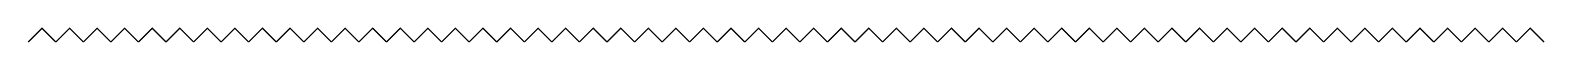
\begin{tikzpicture}[scale=0.35]
\foreach \x in {1,...,55}{
	\draw (\x,-0.25)--(\x+0.5,0.25)--(\x+1,-0.25);
}
\end{tikzpicture}
}

\usepackage{tikz}

\title{\textbf{ Examples:  Quadratic Reciprocity}}
\author{John D Mangual}
\date{}
\begin{document}

\fontfamily{qag}\selectfont \fontsize{25}{30}\selectfont

\maketitle

\noindent Analytic number theory is not my expertise.  Here we work out some softball examples related to quadratic reciprocity. \\ \\
Here's a question: \textbf{Can permutations be used to prove Artin reciprocity} or even parts of Class Field Theory? \\ \\
The proof of quadratic reciprocity seems like a random hodge-podge of techniques.\footnote{This is great for a first class when I was 15 years old it is not so great when you in graduate school are trying to learn Class Field Theory.} Can we unify some of these arguments using:
\begin{itemize}
\item Geometry of Numbers
\item Pigeonhole Principle
\end{itemize}
Gauss in his \textit{Disquiciones Arithmeticae} uses Pigeonhole to prove that $a^p \equiv 0 \mod p$. 

\newpage 

\noindent Any other applications? \\
\begin{tikzpicture}
\draw (0,0)--(19,0);
\end{tikzpicture} \\
Quadratic Reciprocity is stated in the number theory of textbook by \textbf{Hardy + Wright} in a Chapter called 
\begin{center} {\color{green!80!white}Fermat's Theorem and its Consequences}\end{center} \textit{after} his discussion of other more advanced topics
\begin{itemize}
\item prime numbers
\item Farey fractions
\item irrational numbers
\item congruences
\end{itemize}
I dislike prime number theory.  Papers in that subject are quite tedious to read.\\ 
\begin{tikzpicture}
\draw (0,0)--(19,0);
\end{tikzpicture} \\
\\
Fermat's little theorem says, e.g. $27| 3^{27}-1$:
$$ a^p = a \mod p$$
a theorem that I really like is that $5 = 2^2 + 1^2$:
$$ p = a^2 + b^2 \iff p = 4k+1 $$

\newpage

\newpage  

\noindent For proof of Quadratic Reciprocity I always refer to
\begin{itemize}
\item John Conway, \textbf{The Sensual Quadratic Form}
\end{itemize}
and he will use a proof by Zolotarev, involving the permutation group. \\ \\
So let's get started.

\newpage

\fontfamily{qag}\selectfont \fontsize{12}{10}\selectfont


\begin{thebibliography}{}

\item Jared Weinstein. \textbf{Reciprocity laws and Galois representations: recent breakthroughs} Bull. Amer. Math. Soc. 53 (2016), 1-39 

\item David A Cox. \textbf{Primes of the Form $x^2+ny^2$: Fermat, Class Field Theory, and Complex Multiplication} Wiley, 2013.

\item \textbf{A prime ideal $\mathfrak{p}$ decomposes in $\mathbb{Q}(\zeta_{24})/\mathbb{Q}(\sqrt{-6})$ iff it is generated by $\alpha\in1+2\Bbb{Z}[\sqrt{-6}]$} \\ \texttt{http://mathoverflow.net/q/234570/1358}

\item Roy L. Adler \textbf{Symbolic dynamics and Markov partitions}  Bull. Amer. Math. Soc. 35 (1998), 1-56  \\ \texttt{http://www.ams.org/journals/bull/1998-35-01/S0273-0979-98-00737-X/}


\end{thebibliography}



\end{document}